\chapter[Cloud Capacitor]{Cloud Capacitor}
% ----------------------------------------------------------
A partir da especificação do processo de avaliação de capacidade descrita no
capítulo anterior, bem como dos componentes de suporte a esse processo, apresentamos
a sua implementação na forma de um sistema computacional que demonstra seu funcionamento,
eficácia e eficiência.

Cloud Capacitor é um arcabouço para criação de sistemas de avaliação de 
capacidade em ambientes de nuvem de infraestrutura como serviço. Ele permite que 
sejam implementadas lógicas customizadas de avaliação do desempenho resultante
da execução da Aplicação sob Teste. Essas lógicas são então reconhecidas pelo Cloud 
Capacitor como Estratégias de Avaliação.

\begin{figure}[htb]
  \caption{\label{fig_arq_alto_nivel}Arquitetura de alto nível do Cloud Capacitor}
  \begin{center}
    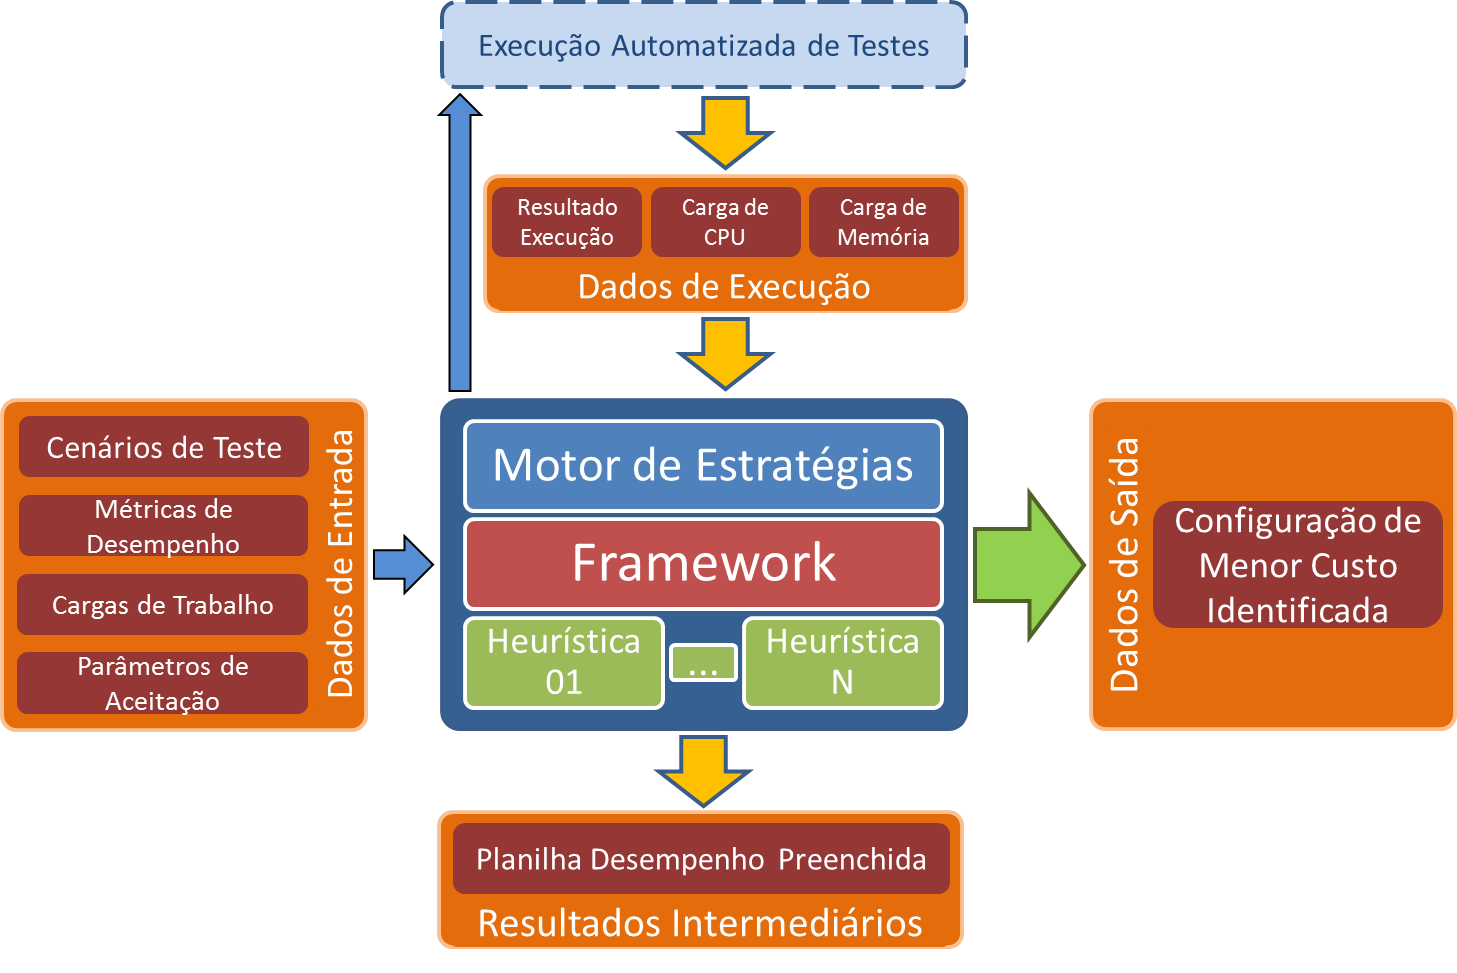
\includegraphics[scale=0.5]{img/arquiteturaAltoNivel}
  \end{center}
\end{figure}
 
% ----------------------------------------------------------
